% !TEX root = SystemTemplate.tex

\chapter{Overview and concept of operations}

This report covers the project overview, user stories, backlog, design and implementation, development environment, deployment, and documentation for the testing project. 


\section{Scope}
This document covers the details of the project including its functionality, tools used, and the process that led to a solution.


\section{Purpose}
The purpose of this program is to run an entire directory of {\tt .cpp} files with given test files, and grade them. There are certain test that are labeled as the critical tests; if a {\tt .cpp} file does not pass one of the critical ones, there is no grade assigned. Otherwise, the percentage of passed test are calculated. 


\subsection{Traversing Subdirectories}
Traversing subdirectories is one of the main components of this system. The program runs a {\tt .cpp} file using test files, and the test files are stored in the same directory as student subdirectories.  

\subsection{Running the Program Using Test Cases}
The software was designed in the Linux environment provided to the group by the university. 

\subsection{Generating Test Cases}
The software is capable of generating test cases if the user provides the constraints. 
 
\section{Systems Goals}
The goal of this system is to make grading a less of a tedious task. This product grades an entire directory of {\tt .cpp} files just by running the root directory. The product is built to test the {\tt .cpp} file with all the given {\tt .tst} test files in the current directory, and compare the results to the corresponding {\tt .ans} files.  

\section{System Overview and Diagram}
Here is a flow diagram showing the implementation process:


\begin{figure}[h]
\centering 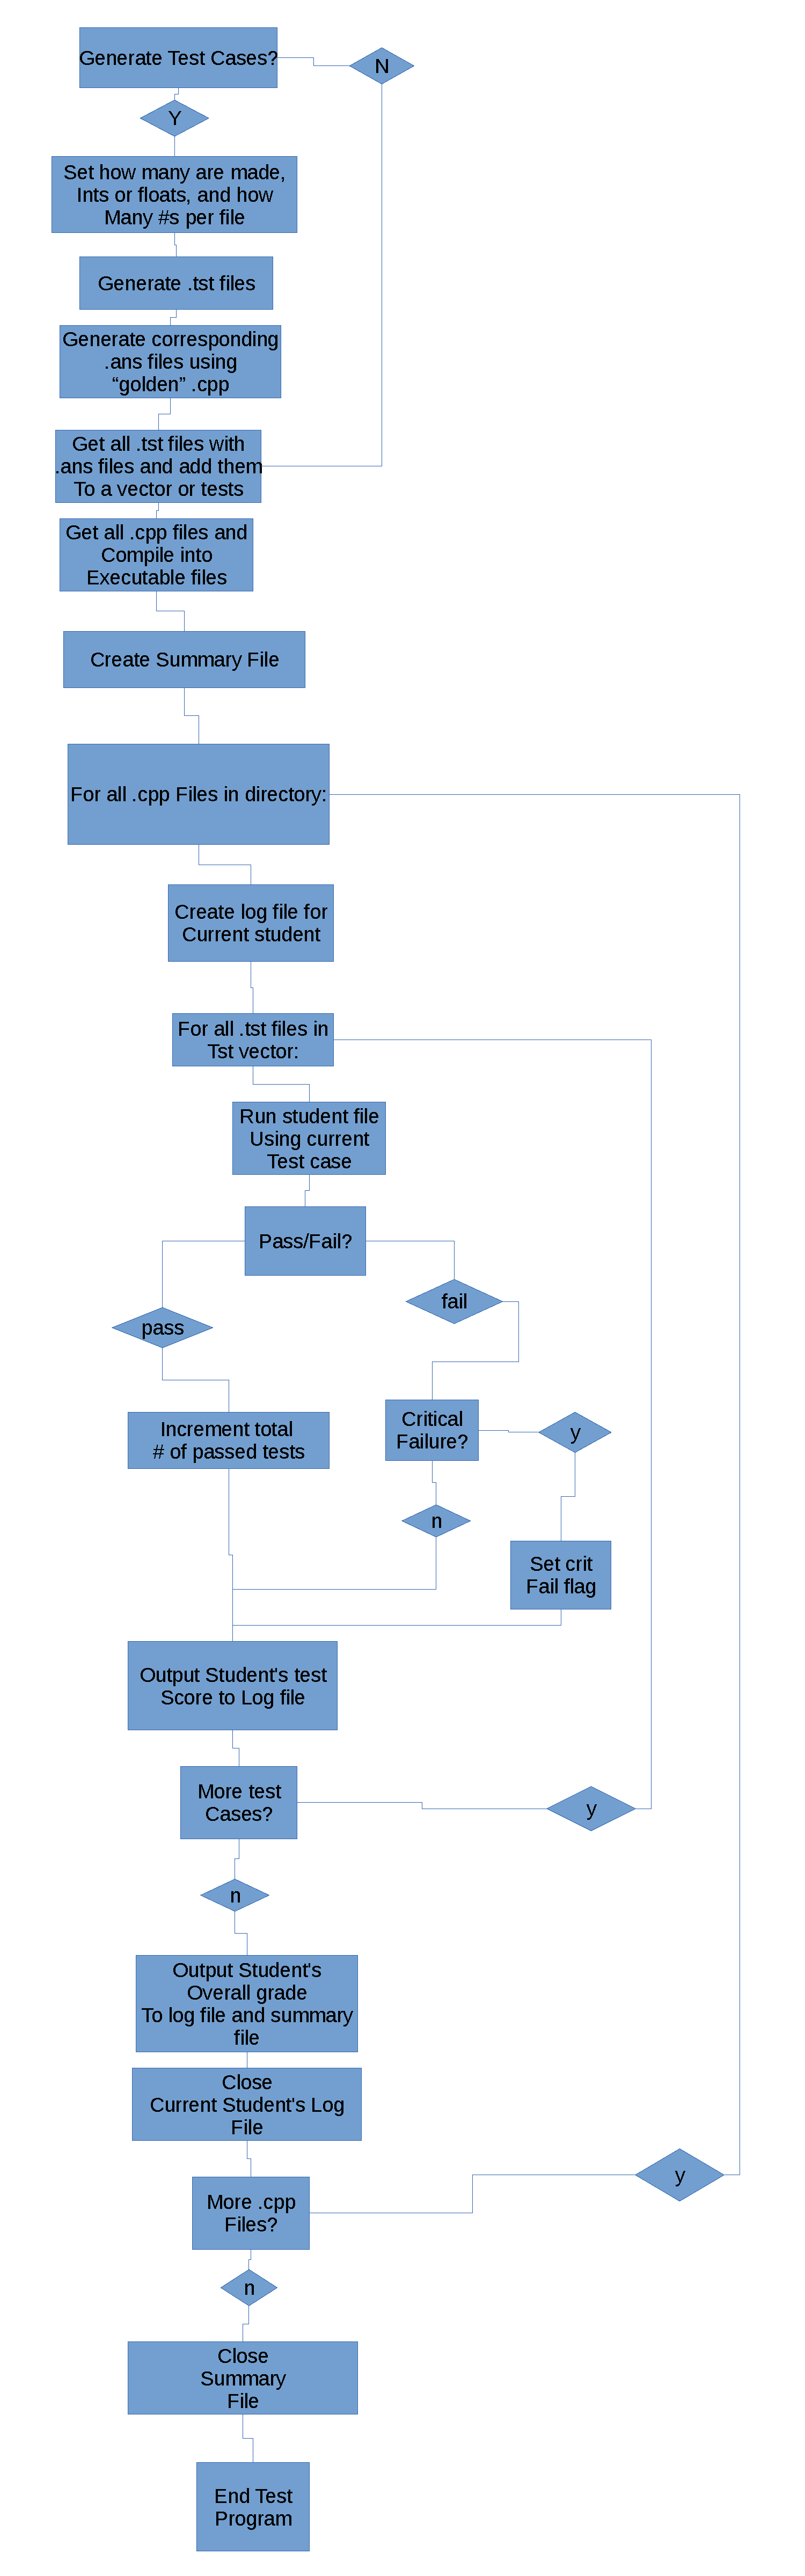
\includegraphics[width=7cm]{sprint2Algorithm}
\end{figure}

\let\cleardoublepage\clearpage


